
\documentclass{article}
\usepackage[ascii]{inputenc}
\usepackage[T1]{fontenc}
\usepackage[english]{babel}
\usepackage{amsmath}
\usepackage{amssymb,amsfonts,textcomp}
% \usepackage{mathtools} % added by mjirik
% \usepackage{siunitx}
\usepackage{fancyvrb}
\usepackage{color}
\usepackage{array}
\usepackage{supertabular}
\usepackage{hhline}
\usepackage[normalem]{ulem}
\usepackage{hyperref}
\usepackage{textcomp}
\usepackage{layout}
\usepackage[numbers]{natbib}
\usepackage{caption}

\usepackage{hyperref}
\newcommand{\doi}[1]{\href{http://dx.doi.org/#1}{\nolinkurl{#1}}}
% \newcommand{\doi}[1]{\textsc{doi}: \href{http://dx.doi.org/#1}{\nolinkurl{#1}}}

\hypersetup{colorlinks=true, linkcolor=black, citecolor=black, filecolor=blue, urlcolor=blue, pdftitle=CAD17abstract, pdfauthor=Orest Mykhaskiv, pdfsubject=, pdfkeywords=}
\usepackage[pdftex]{graphicx}

\newcommand\textstyleInternetlink[1]{\textcolor{blue}{#1}}

\setcounter{secnumdepth}{2}
\renewcommand\thesection{\arabic{section}}
\renewcommand\thesubsection{\arabic{section}.\arabic{subsection}}
\makeatletter
\newcommand\arraybslash{\let\\\@arraycr}
\makeatother

\newcommand\liststyleWWviiiNumxxxiii{%
\renewcommand\labelitemi{{\textbullet}}
\renewcommand\labelitemii{{}-}
\renewcommand\labelitemiii{${\blacksquare}$}
\renewcommand\labelitemiv{{\textbullet}}
}
\newcommand\liststyleWWviiiNumxxix{%
\renewcommand\labelitemi{{\textbullet}}
\renewcommand\labelitemii{o}
\renewcommand\labelitemiii{${\blacksquare}$}
\renewcommand\labelitemiv{{\textbullet}}
}
\newcommand\liststyleWWviiiNumxxiv{%
\renewcommand\labelitemi{{\textbullet}}
\renewcommand\labelitemii{o}
\renewcommand\labelitemiii{${\blacksquare}$}
\renewcommand\labelitemiv{{\textbullet}}
}
\newcommand\liststyleWWviiiNumxxi{%
\renewcommand\labelitemi{{\textbullet}}
\renewcommand\labelitemii{o}
\renewcommand\labelitemiii{${\blacksquare}$}
\renewcommand\labelitemiv{{\textbullet}}
}
\newcommand\liststyleWWviiiNumxxiii{%
\renewcommand\labelitemi{{\textbullet}}
\renewcommand\labelitemii{o}
\renewcommand\labelitemiii{${\blacksquare}$}
\renewcommand\labelitemiv{{\textbullet}}
}
\newcommand\liststyleWWviiiNumxv{%
\renewcommand\labelitemi{{\textbullet}}
\renewcommand\labelitemii{o}
\renewcommand\labelitemiii{${\blacksquare}$}
\renewcommand\labelitemiv{{\textbullet}}
}
\newcommand\liststyleWWviiiNumxxx{%
\renewcommand\theenumi{\arabic{enumi}}
\renewcommand\theenumii{\alph{enumii}}
\renewcommand\theenumiii{\roman{enumiii}}
\renewcommand\theenumiv{\arabic{enumiv}}
\renewcommand\labelenumi{[\theenumi]}
\renewcommand\labelenumii{\theenumii.}
\renewcommand\labelenumiii{\theenumiii.}
\renewcommand\labelenumiv{\theenumiv.}
}
\newcommand\liststyleWWviiiNumxxxii{%
\renewcommand\labelitemi{{\textbullet}}
\renewcommand\labelitemii{o}
\renewcommand\labelitemiii{${\blacksquare}$}
\renewcommand\labelitemiv{{\textbullet}}
}

\renewcommand\refname{}
\renewcommand{\bibsection}{}
\renewcommand{\theequation}{2.\arabic{equation}}


\setlength\paperwidth{19.05cm}
\setlength\paperheight{26.162cm}
\setlength\voffset{-1in}
\setlength\hoffset{-1in}
\setlength\topmargin{30pt}
\setlength\oddsidemargin{1.524cm}
\setlength\textheight{576pt}
\setlength\textwidth{16.001999cm}
\setlength\footskip{0.841cm}
\setlength\headheight{16pt}
\setlength\headsep{28pt}


\usepackage{fancyhdr}
\pagestyle{fancy}
\fancyhf{}
\renewcommand{\headrulewidth}{0pt}
\renewcommand{\footrulewidth}{0.4pt}
\fancyhead[R]{\thepage}
\fancyfoot[R]{Proceedings of CAD'20, Barcelona, Spain, July 6-8, 2020, aaa-bbb\\ {\footnotesize{\textcopyright}} 2020 CAD Solutions, LLC, \ULurl{http://www.cad-conference.net}}

\usepackage{etoolbox}
\patchcmd{\thebibliography}{\section*{\refname}}{}{}{}
\captionsetup[figure]{labelformat={default},name={Fig.}}

\setlength{\bibsep}{2pt plus 0.3ex}
\setcounter{page}{1}

\makeatletter
\DeclareUrlCommand\ULurl@@{%
  \def\UrlFont{\ttfamily\color{blue}}%
  \def\UrlLeft{\uline\bgroup}%
  \def\UrlRight{\egroup}}
\def\ULurl@#1{\hyper@linkurl{\ULurl@@{#1}}{#1}}
\DeclareRobustCommand*\ULurl{\hyper@normalise\ULurl@}
\makeatother

% defined by mjirik
\newcommand{\E}{\mathbb{E}}
\newcommand{\B}{\mathbb{B}}
\newcommand{\N}{\mathbb{N}}

\begin{document}

{\centering  
\includegraphics[width=5.173cm,height=2.193cm]{images/CADconverted-img001.jpg} \par}

\vspace{5pt}
\noindent
\underline{Title:}

\noindent{\bfseries
Algebraic Filtering of Surfaces from 3D Medical Images with Julia
% Word Template for CADxx Extended Abstracts
}

\vspace{1em}
\noindent \underline{Authors:}
\newline
Miroslav Jirik, jirik@lfp.cuni.cz, Charles University\newline
Alberto Paoluzzi, paoluzzi@dia.uniroma3.it, Roma Tre University
% John C. Gotti, gotti@cityuny.edu, City University of New York \newline
% Jessie A. James, Jessie@tsu.edu, Texas State University \newline
% Donald L. Corleone, don@dlc.com, 3DLC and Associates

\vspace{1em}
\noindent \underline{Keywords:}\newline
Medical 3D, Computational Topology, Linear Algebraic Representation, LAR, Julia, Surface Extraction
% Rapid Prototyping, FDM, Z-Printer, Surface Finish, Dimensional Accuracy, Process Optimization


\bigskip


\noindent \underline{DOI:} 10.14733/cadconfP.2020.xxx-yyy

\vspace{10pt}
\noindent\underline{Introduction:}\vspace{0.2em}\newline
In this paper we introduce a novel algebraic \textsc{lar-surf} (Linear Algebraic Representation Surface extraction) filter, well founded on algebraic topology methods, to extract and smooth the boundary surface of any subset of voxels arising from the segmentation of a 3D medical image.

Isosurface extraction to produce geometric models of surfaces from volumetric data 
% is important in many applications. It 
is often used for indirect visualization of the medical data or for flow modeling. % \cite{Rohan2018a}. 
% In this paper
Here we discuss an approach based on basic algebraic topology and linear algebra, using linear spaces $C_p$ of chains (of cells) of dimension $0 \leq p \leq 3$ and the boundary matrix $[\partial_3] : C_3 \to C_2$.

Input volumetric data are represented by a 3D voxel array and can be generated by segmentation computed tomography (Fig. \ref{fig:liver} left) and they are defined as a \emph{chain}, i.e. as a vector from a linear space $C_3$ of 3-chains, represented in coordinates as a sparse binary vector.

A decomposition of the input volumetric data into small submatrices called ``bricks'' is performed, then the binary coordinate vector of each interesting chain of voxels is generated, and its boundary is computed by matrix multiplication times the boundary matrix producing the binary representation of the boundary surface (surface which define boundary). % TODO {explain boundary surface}
The output is produced by a linear mapping between spaces of 3- and 2-chains through the boundary operator $\partial_3:C_3 \to C_2$.  In particular, when the input set of voxels is either not (4-)connected, or contains one or more empty regions inside, \textsc{lar-surf} generates a non-connected set of closed surfaces, i.e. a triangle faces (Fig. \ref{fig:schema}). % or a set of 2-cycles---using the language of algebraic topology. 
%The only data structures used by this approach are sparse arrays with one or two indices, i.e.~sparse vectors and matrices. 


Parallel data decomposition is used to compute the boundary surface patches within each of the bricks, that are finally joined and smoothed via the Taubin algorithm 
\cite{Taubin:1995:SPA:218380.218473}
This work is based on LAR (Linear Algebraic Representation) methods 
\cite{DiCarlo2009,DiCarlo2014}
%ieee-tase, 
% DBLP:journals/cad/DiCarloPS14
% DBLP:journals/cad/DiCarloPS14
, and is implemented in Julia language, natively supporting parallel computing on hybrid hardware architectures.

\vspace{10pt}
\noindent\underline{
Representation Scheme:}\vspace{0.2em}\newline
With \emph{Boundary representations} (`$B$-reps'), where the solid model is represented through a representation of its boundary elements, i.e.~faces, edges and vertices;
\emph{decompositive/enumerative representations} \cite{Requicha:1980:RRS:356827.356833}, are a decomposition of either the object or the embedding space, respectively, into a well-defined \emph{cellular complex}. In particular, a boundary representation provides a cellular decomposition of the object's boundary into \emph{cells} of dimension zero (vertices), one (edges), and two (faces). Medical imaging can be classified as the \emph{enumerative representation} of cellular decompositions of organs and tissues of interest \cite{Paoluzzi2016}, in particular, as subsets \emph{of 3D volume elements} (voxels) from the 3D image. 

% The 
\textsc{LAR}
% , introduced in~ % \cite{Dicarlo:2014:TNL:2543138.2543294}
% \cite{DiCarlo2014},
aims to represent the \emph{chain complex}~\cite{TSAS} generated by a piecewise-linear \emph{geometric complex} embedded either in 2D or in 3D. 
In a few words, it gets a minimal characterization of geometry and topology of a cellular complex, i.e.~the embedding mapping $\mu : C_0 \to \E^d$ of 0-cells (vertices), as well a description of $(d-1)$-cells as subsets of vertices, and is able to return the whole chain complex 
% \begin{equation}
\[
C_\bullet = (C_p, \partial_p) := 
C_3 
\substack{
\delta_2 \\
\longleftarrow \\
\longrightarrow \\
\partial_3 
}
C_2 
\substack{
\delta_1 \\
\longleftarrow \\
\longrightarrow \\
\partial_2 
}
C_1  
\substack{
\delta_0 \\
\longleftarrow  \\
\longrightarrow \\
\partial_1 
}
C_0 .
\]
% \end{equation}
\noindent
and, in particular, any basis for linear chain spaces $C_p$, and any linear
boundary/coboundary map \(\partial_p\) and
\(\delta_p=\partial_{p-1}^\top\) between them. The \emph{domain} of \textsc{lar} is the set of \textbf{chain complexes} generated by cell $d$-complexes ($2\leq d\leq 3$). 
% The computer \emph{representations} of \textsc{lar} are \textbf{sparse binary matrices} to represent both the operators and the chain bases. 
In algebraic topology a $p$-chain is defined as a linear combination of $p$-cells with scalars from a field. 
% When the scalar coefficients are from $\{-1, 0, +1\}$, a chain may represent \emph{any (oriented) subset of cells} from the cellular complex. 
%
% Scalars from $\{0, 1\}$ are used for non-oriented complexes.
We may get the $(p-1)$-boundary $\partial_p c_p$ of \emph{any} $p$-chain $c_p$, by multiplication of the coordinate representation $[\partial_p]$ of the boundary operator times the coordinate representation $[c_p]$ of the chain in terms of such scalars, i.e.~by a  matrix-vector product $ [\partial_p] [c_p] $.

The geometry and topology required to display (Fig. \ref{fig:liver}) a triangulation of boundary faces
% To display a triangulation of  boundary faces  in their proper position in space, the information required (geometry and topology) 
is contained in the \emph{geometric chain complex} \texttt{(geom, top) = (V, (EV, FE, CF))},
% TODO remove ?
% . This pair is equivalent to the embedding function $\mu: C_0  C_0\to\E^3$ and by the coboundary chain ($\delta_0, \delta_1, \delta_2$)
where the geometry \texttt{geom} is given by
the embedding matrix \texttt{V} of vertices (0-cells), and  topology \texttt{top} by the three sparse matrices (\texttt{EV}, \texttt{FE}, \texttt{CF}) of coboundaries ($\delta_0, \delta_1, \delta_2$) of the chain complex (Fig. \ref{fig:boundary_matrix_4x4x4}). The ordered pairs of letters from \texttt{V,E,F,C}, correspond to \emph{\emph{\texttt{V}}ertices$\to$\emph{\texttt{E}}dges$\to$\emph{\texttt{F}}aces$\to$\emph{\texttt{C}}ells} into the 
\emph{\emph{\texttt{C}}olumn$\to$\emph{\texttt{R}}ow} order of matrix maps of operators.

\begin{figure}[tbp] %  figure placement: here, top, bottom, or page
   \centering
   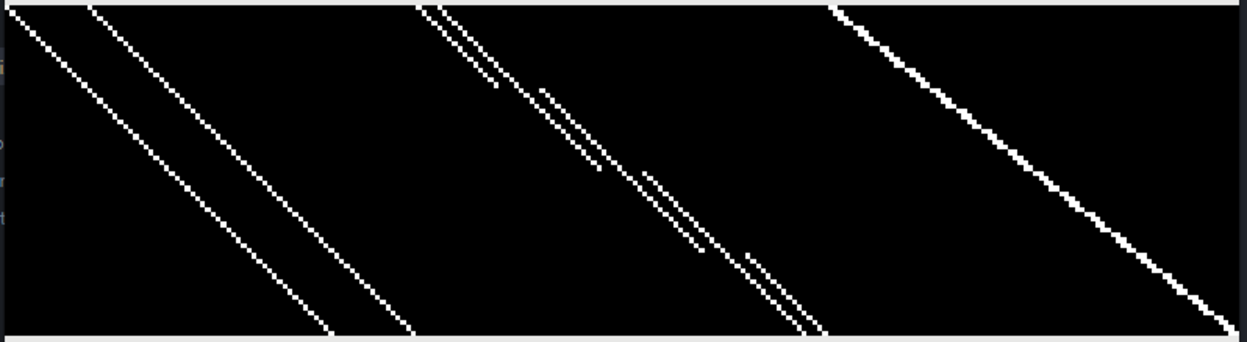
\includegraphics[width=0.76\linewidth]{figs/boundary_matrix_4x4x4.pdf} 
   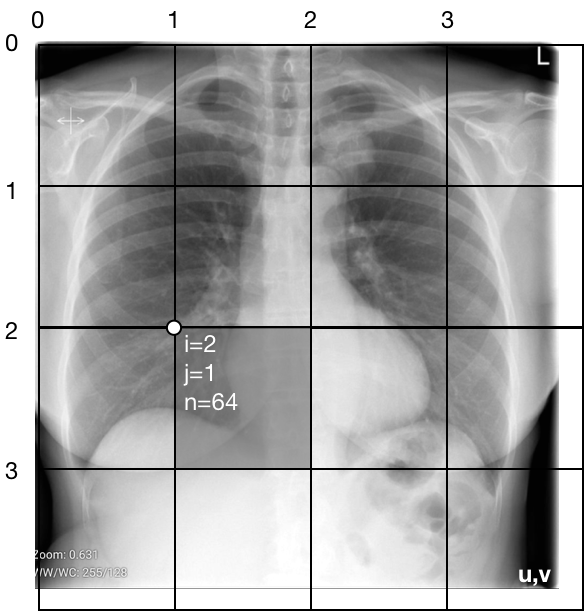
\includegraphics[width=0.22\linewidth]{figs/blocks} 
  \caption{
Left image: the binary image of coboundary matrix 
% $\left[\delta_2\right]
% = \left[\partial_3\right]^t : C_2 \to C_3$, 
  built for a small volumetric data/brick with shape $(4,4,4)$. The number of rows is $4\times 4\times 4$; the number of columns is $d\,n\,(1+n)^{d-1} = 3\times 4\times 25$. \\
%   Of course, the number of non-zeros per row (cardinality of the facet set of a single voxel) is six, whereas the number of non-zeros per column is two, but on boundary facets.
   The right image shows a possible brick partitioning of a radiologic image. The evidenced 2D brick, of size $n^d=64^2$, is sliced by $\B([2,1,64]) = image([128:172],[64:128)]$
   }
   \label{fig:boundary_matrix_4x4x4}
\end{figure}

% \begin{figure}[htbp] %  figure placement: here, top, bottom, or page
%   \centering
%   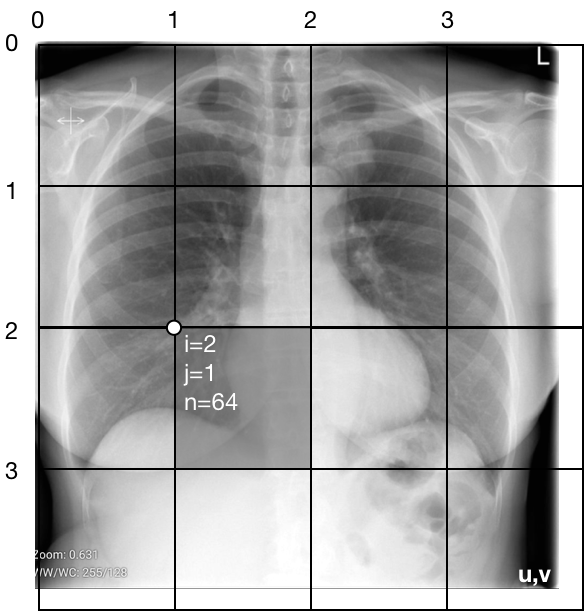
\includegraphics[width=0.5\linewidth]{figs/blocks} 
%   \caption{A possible brick partitioning of a radiologic image. The evidenced 2D brick, of size $n^d=64^2$, is sliced by $\B([2,1,64]) = Image([128:172],[64:128)]$}
%   \label{fig:blocks}
% \end{figure}

\vspace{10pt}
\noindent\underline{
Construction of boundary matrix  $\partial_d$:}\vspace{0.2em}\newline 
First, let us fix an ordering for all the cells of a partition of input data (with vertices $V$, edges $E$, pixels $F$, and voxels $C$) i.e.~for each 0-, 1-, 2-, and 3-cell. These orderings define the $p$-bases for the linear spaces $C_p$ of $p$-chains $(0 \leq p \leq 3)$. 
We call $M_p=\left(m_{i,j}\right)$ the binary
\emph{characteristic matrix} of the $p$-basis, expressed as subsets so that $m_{i,j}=1$ if and only if the $j$-th  $0$-cell $c^j_0$ belongs 
% , where  we have that $m_{i,j}=1$ if and only if the $j$-th $0$-cell belongs 
to the boundary of $i$-th $p$-cell $m_{i,j}$, and $m_{i,j}=0$ otherwise. 

The product of binary matrices is not binary.
% , so by computing the (sparse) matrix product $(M_{p-1} M_{p}^t) = (n_{i,j})$, with $n_{i,j} = \sum_{k} m_{i,k}m_{k,j}$, we get for each $n_{ij}$ the \emph{number of vertices} shared by $c_{p-1}^i$ and $c_{p}^j$. When this number equates the cardinality of $c_{p-1}^i$, this elementary chain is contained on the boundary of $c_{p}^j$. 
In a 3D image, with cubic 3-cells and squared 2-cells in-between, 
% everywhere we get $n_{i,j}=4$, we 
% may state $c_{2}^i\subset\partial c_{3}^j$. In each $j$ column of $M_{2} M_{3}^t = (n_{i,j})$, 
we 
have exactly \emph{six rows} where  $n_{i,j} = 4$, since a cube (3-chain) has six boundary faces (2-chains). The unit incidence coefficients in $\left[\partial_3\right]$ are found by filtering with value 4.
% The binary image of coboundary matrix

\begin{figure}
\centering
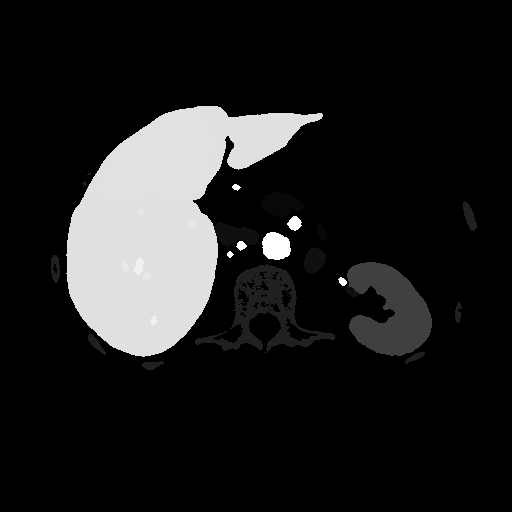
\includegraphics[width=0.25\textwidth]{figs/ircad01_segmentation_65.png}%
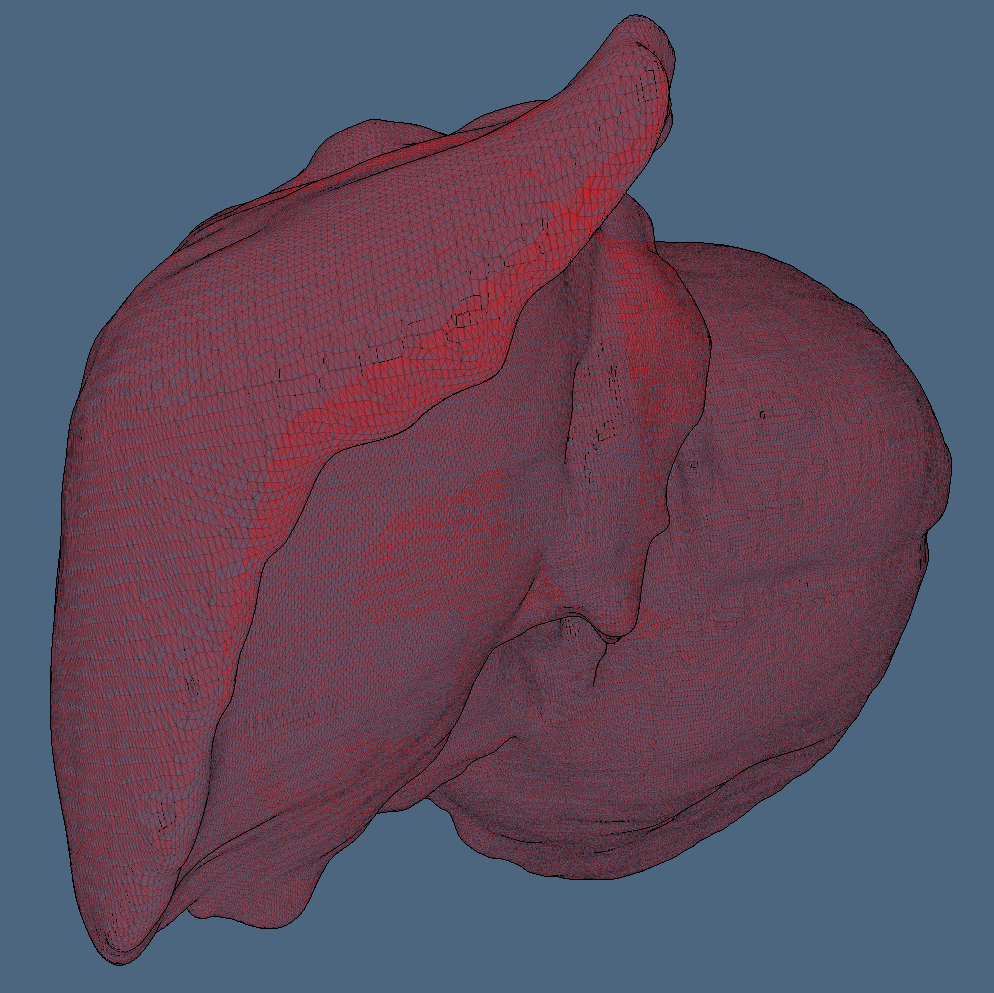
\includegraphics[width=0.25\textwidth]{figs/liver_01_red_3.png}%
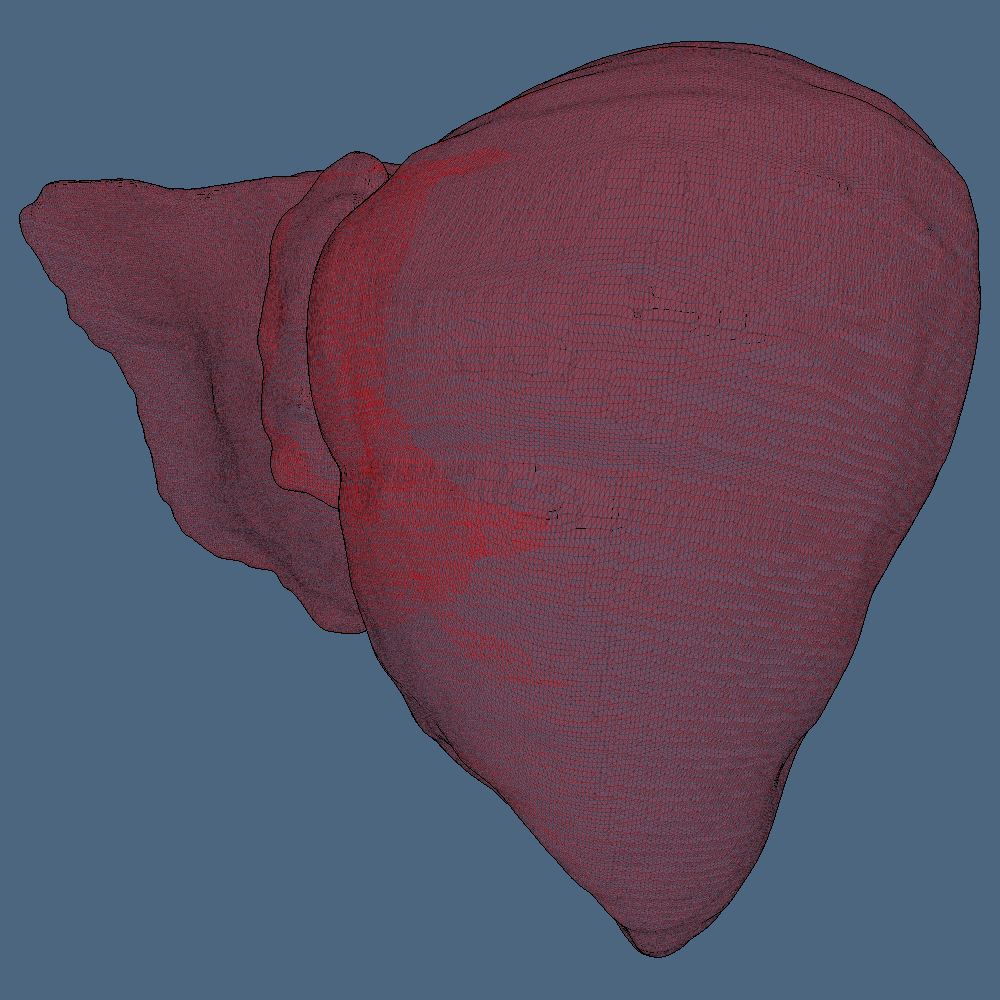
\includegraphics[width=0.25\textwidth]{figs/liver_01_red_4.png}%
% 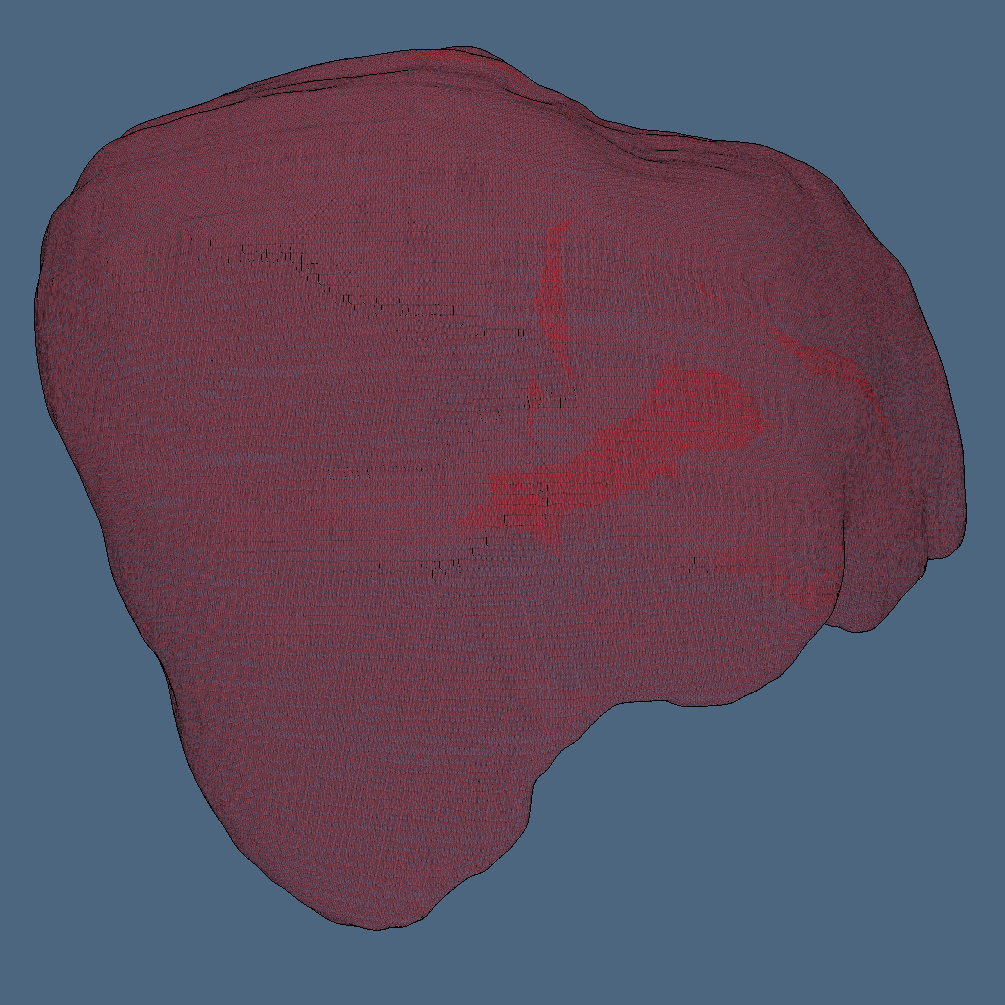
\includegraphics[width=0.24\textwidth]{figs/liver_01_red_5.png} 
% \vspace{0.05\textwidth}
% \includegraphics[width=0.24\textwidth]{figs/portalvein_01_yellow_3.png} 
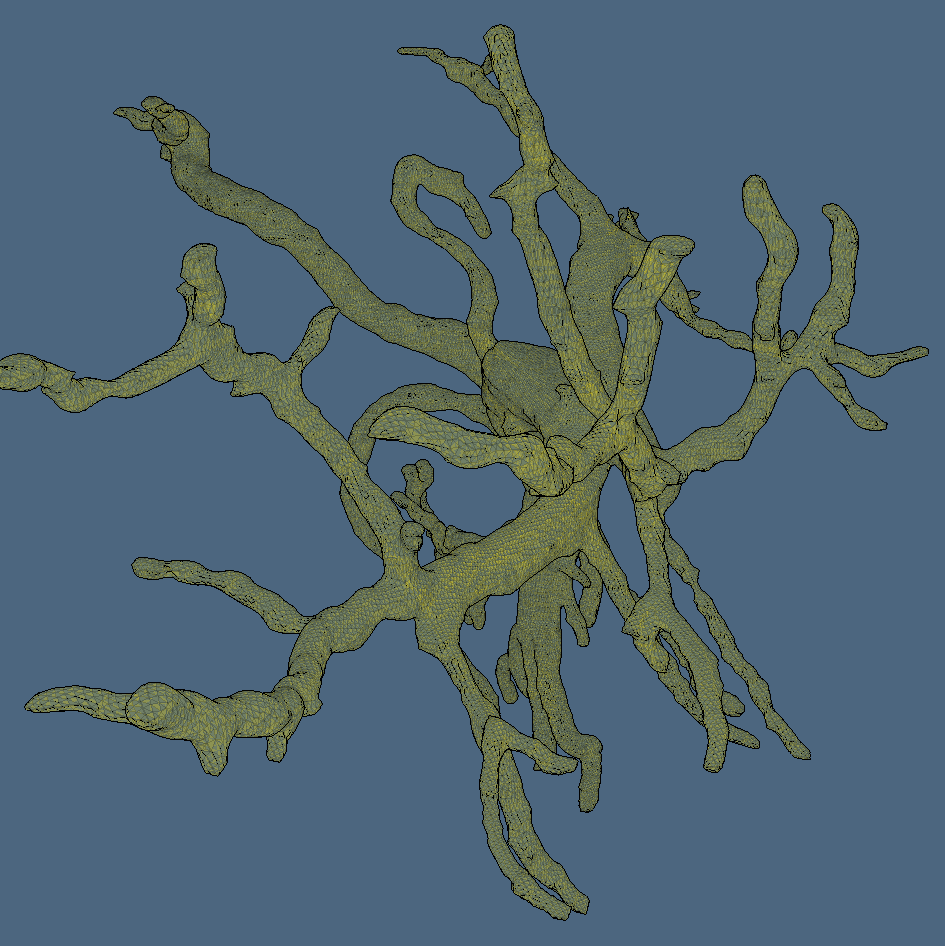
\includegraphics[width=0.25\textwidth]{figs/portalvein_01_yellow_2.png} 
% \vspace{0.01\textwidth}
% \includegraphics[height=0.24\textwidth]{src/figs/nrn10_100_magenta_high_res.png} 
% \includegraphics[height=0.4\textwidth]{figs/nrn10_100_low_res.png} 
% \vspace{0.05\textwidth}
% \includegraphics[width=0.24\textwidth]{figs/porta_smoothing_2.png} 
% of the input volumetric data 
\caption{
The left image shows one slice 
with segmented organs from 
the Ircad dataset \cite{ircad}. The other three images show the surface of the liver and portal vein generated by \texttt{lar-surf.jl} package.
} \label{fig:liver}
\end{figure}
% Triangulated isosurface of liver parts extracted with LAR-SURF algorithm. 
% On the upper left image the surface of the liver parenchyma of human can be seen. 
% Both right images show the Portal Vein from the same 
% with resolution $1.6\times0.57\times0.57$ [mm].
% On the left bottom image is the pig liver microvasculature based on corrosion cast prepared by Eberlova
% \cite{eberlova2017use}. The resolution of the Micro-CT data is 4.682 $\mu{}m$.

\vspace{10pt}
\noindent\underline{
Example: Boundary matrices for grids of cubes:
}\vspace{0.2em}\newline 
% NOTE this is new 
We give here the full Julia code for the algebraic computation of $\partial_3$ matrix, for a very little grid of unit
3-cubes. Due to the simplicity of the cells (voxels = cubes), a sufficient (geom,top) pair is given below
as (\texttt{V,CV}), where \texttt{CV} is an array of arrays of \texttt{Float64} indices of grid cubes.

% julia> V
% 3x24 Array{Float64,2}:
% julia> CV
% 6-element Array{Array{Int64,1},1}:
\begin{Verbatim}[fontsize=\footnotesize]
julia> V, CV = Lar.cuboidGrid([3,2,1])
julia> V
0.0 0.0 0.0 0.0 0.0 0.0 1.0 1.0 1.0 1.0 1.0 1.0 2.0 2.0 2.0 2.0 2.0 2.0 3.0 3.0 3.0 3.0 3.0 3.0
0.0 0.0 1.0 1.0 2.0 2.0 0.0 0.0 1.0 1.0 2.0 2.0 0.0 0.0 1.0 1.0 2.0 2.0 0.0 0.0 1.0 1.0 2.0 2.0
0.0 1.0 0.0 1.0 0.0 1.0 0.0 1.0 0.0 1.0 0.0 1.0 0.0 1.0 0.0 1.0 0.0 1.0 0.0 1.0 0.0 1.0 0.0 1.0
julia> CV
[[ 1, 2, 3, 4, 7, 8, 9,10], [ 3, 4, 5, 6, 9,10,11,12], [ 7, 8, 9,10,13,14,15,16],
 [ 9,10,11,12,15,16,17,18], [13,14,15,16,19,20,21,22], [15,16,17,18,21,22,23,24]
\end{Verbatim}

\vspace{10pt}
\noindent\underline{
Face and Edge Data generation:
}\vspace{0.2em}\newline 
%TODO describe CV2FV and CV2EV
In the following, we provide the functions for generating the face data \texttt{FV} (vertex indices in faces) with function  \texttt{CV2FV} and edge data \texttt{EV} (vertex indices in edges) with function \texttt{CV2EV} from cell data \texttt{CV}. 
% In particular,  and  functions apply to all the 3-cells in \texttt{CV} the pattern of reference to vertices used by faces and edges of the single 3-cube:



% \footnotesize
%\small]
\begin{Verbatim}[fontsize=\footnotesize]
function CV2FV( v:: Array { Int64 } )
return faces = [[v[1], v[2], v[3], v[4]], [v[5], v[6], v[7], v[8]],
                [v[1], v[2], v[5], v[6]], [v[3], v[4], v[7], v[8]],
                [v[1], v[3], v[5], v[7]], [v[2], v[4], v[6], v[8]]]
end
function CV2EV( v:: Array { Int64 } )
return edges = [[v[1],v[2]], [v[3],v[4]], [v[5],v[6]], [v[7],v[8]], [v[1],v[3]], [v[2],v[4]],
                [v[5],v[7]], [v[6],v[8]], [v[1],v[5]], [v[2],v[6]], [v[3],v[7]], [v[4],v[8]]]
end
\end{Verbatim}

\vspace{10pt}
\noindent\underline{
Characteristic matrices:
}\vspace{0.2em}\newline 
The function \texttt{K} transforms an array of arrays ($\mathtt{VV, EV, FV, CV}$) into a sparse binary characteristic matrix
($\mathtt{M_0, M_1, M_2, M_3}$). A Julia sparse matrix needs three arrays I, J, Vals of rows, columns, values of non-zeros:

% VV = [[v] for v=1:size(V, 2)]
% [1],[2],[3],[4],[5],[6],[7],[8],[9],[10],[11],[12],[13],[14],[15], [16],[17],
% [18],[19],[20],[21],[22],[23],[24]
% [1],[2],[3],[4],[5],[6],[7],[8],[9],[10],[11],[12],[13],[14],[15], [16],[17],
% [18],[19],[20],[21],[22],[23],[24]
\begin{Verbatim}[fontsize=\footnotesize]
VV = [[v] for v=1:size(V, 2)];
FV = collect(Set{Array{Int64,1}}(cat(map(CV2FV, CV))))
[[13,15,19,21], [1,2,3,4], [7,9,13,15], [13,14,15,16], [7,8,13,14], [1,2,7,8], [2,4,8,10], [7,8,9,10], 
 [3,5,9,11], [8,10,14,16], [15,16,21,22], [9,11,15,17], [3,4,5,6], [17,18,23,24], [11,12,17,18], 
 [1,3,7,9], [3,4,9,10], [9,10,15,16], [4,6,10,12], [13,14,19,20], [9,10,11,12], [15,16,17,18], 
 [19,20,21,22], [15,17,21,23], [16,18,22,24], [21,22,23,24], [10,12,16,18], [5,6,11,12], [14,16,20,22]]

EV = collect(Set{Array{Int64,1}}(cat(map(CV2EV, CV))))
[[15,17], [16,22], [6,12], [17,23], [18,24], [4,10], [3,4], [13,15], [11,12], [9,15], [13,19],
 [1,7], [5,11], [5,6], [12,18], [8,14], [15,21], [17,18], [1,3], [2,4], [16,18], [2,8], [21,23],
 [20,22], [1,2], [14,16], [10,16], [13,14], [19,21], [7,13], [9,10], [23,24], [11,17], [21,22],
 [3,9], [3,5], [9,11], [7,9], [14,20], [7,8], [22,24], [19,20], [8,10], [15,16], [10,12], [4,6]]

function K(CV)
    I = vcat ( [ [k for h in CV[k]] for k =1: length (CV) ]...)
    J = vcat (CV ...)
    Vals = Int8 [1 for k=1: length (I)]
    return SparseArrays . sparse (I,J,Vals)
end
M0 = K(VV); M1 = K(EV); M2 = K(FV); M3 = K(CV)
\end{Verbatim}

\vspace{10pt}
\noindent\underline{
Boundary matrices:
}\vspace{0.2em}\newline 
The boundary matrices between non-oriented chain spaces are computed by sparse matrix multiplication
followed by matrix filtering, produced in Julia by the broadcast of vectorized integer division ($.\div$):

% TODO this is strange the M_1 is M_1 after multiplication?
$\partial_1 =  \mathtt{M_0} * \mathtt{M'_1} = \mathtt{M'_1}$

$\partial_2 =  \left(\mathtt{M_1} * \mathtt{M'_2}\right) .\div \mathtt{sum(M_1, dims=2)}$

$\partial_3 =  \left(\mathtt{M_2} * \mathtt{M'_3}\right) .\div \mathtt{sum(M_2, dims=2)}$
\begin{figure}[tbp]
\centering
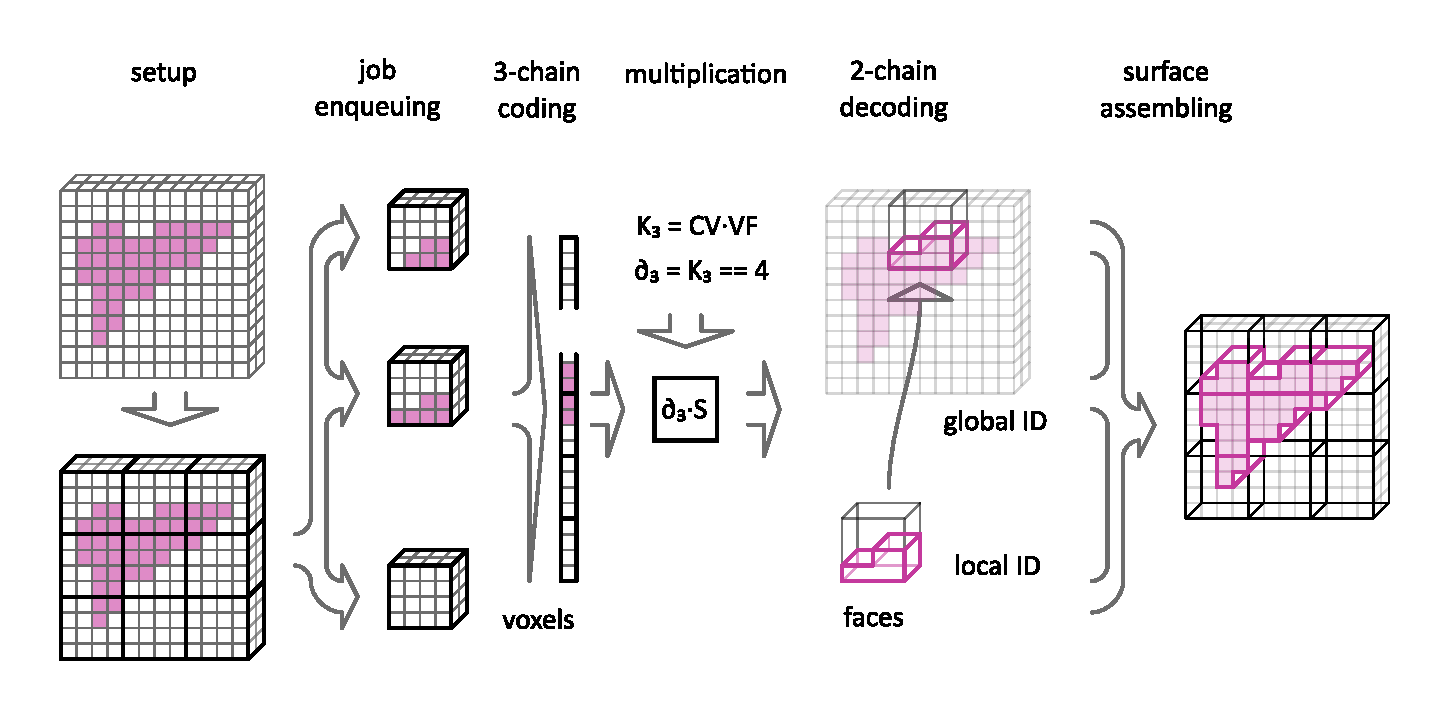
\includegraphics[width=0.9\textwidth]{figs/schema_horizontal.pdf} 
%\includegraphics[scale=1]{input/ircad_comparison.pdf} 
\caption{Workflow of \textsc{lar-surf} algorithm}
\label{fig:schema}
\end{figure}



\vspace{10pt}
\noindent\underline{
Brick-level parallelism:
}\vspace{0.2em}\newline 
Let us assume that medical devices produce 3D images with lateral dimensions that are integer multiples of some powers of two, like 256, 512, etc.
Any cuboidal portion of the image 
$\B$, called \emph{brick},
is completely determined by highest and lowest Cartesian indices of its voxels (Fig. \ref{fig:boundary_matrix_4x4x4} right).
% and extracted by multidimensional array \emph{slicing} as $image([\ell_x : h_x, \ell_y : h_y, \ell_z : h_z])$.
% For the sake of simplicity, 
We assume 
% common size on the three image axes, and the corresponding 
$\B$ as a function of its element of the  lowest  brick coordinates $i,j,k\in \left[1:n\right]$ and 
the brick lateral size $n\in\N$:
\[
\B(i,j,k,n) := image([in:in+n, jn:jn+n, kn:kn+n]) 
\]
% In our computational pipeline
% TODO add linkg to figure 3
% (Fig \ref{fig})
%, several steps can be efficiently performed in parallel at the image-block level.
% , depending on the embarrassingly data-parallel nature of the problem. 
% In particular, 
% Little effort is needed to separate the problem into a several of parallel tasks $S_{i,j,k}$, using multiarray slicing. 
The granularity of parallelism, depending on the block size $n$, is further enforced by the computation of a single boundary matrix $[\partial_d(n)]$ depending on $n$.
% , so that the initial communication cost of broadcasting the matrix to nodes can be carefully controlled, and finely tuned depending on the system architecture. 
% TODO zkracovat


In our experiment we applied the \textsc{lar-surf} filter on 20 segmented volumetric data from dataset Ircad \cite{ircad} with lateral size $512\times512$ and 74 -- 260 slices. We compared the performance of \textsc{lar-surf} with marching-cubes algorithm implemented in Python.
Based on t-test with $\alpha=0.99$, $p=8.74\times10^{-24}$ and 
$s=-16.67$ it can be shown that the mean of time consumed by \textsc{lar-surf} is significantly lower from time consumed by marching-cubes.


\vspace{0.8em}
\noindent\underline{Discussion of method}\vspace{0.2em}\newline
The greatest amount of other methods for extraction of boundary surfaces from 3D data arrays---including~\cite{10.1016/j.cad.2006.09.003} and~\cite{10.1115/1.2960489}---use implicit functions, defined by first averaging upon 3D mesh vertices the lighting or brightness of incident voxels, and then by applying some marching cube algorithm in order to traverse and to triangulate  the iso-valued boundary patches.  

Conversely, we use a binary labeling of the voxel sets of interested image segment, and the standard medical 3D image array as solid representation. The set of boundary facets is extracted through spMV (sparse matrix vector multiplication) of the $[\partial_3]$ matrix times the binary vector labeling the voxels of the segment. The boundary matrix is computed once and for all, sent to all workers (cores or nodes), then used in parallel for all image brick extractions. This algebraic method can be immediately extended to multi-material processing, as well as to design multi-material tissue layering for 3D printing.

In particular, we might organize a multi-material (or multi-organ) extraction, simply by multiplication of the boundary matrix $[\partial_3]: C_3\to C_2$  times a binary matrix where the non-zeros elements on each column represents either one of the materials, or one of the organs to be algebraically extracted by the filter. The two surface patches common to two adjacent segments will be exactly coincident, and share the same geometry and topology, with the only exception of each patch contours, where the influence of adjacent patches induces each instance to be separated and round-off.

To make our algorithm consistent with results given by~\cite{10.1016/j.cad.2006.09.003} and ~\cite{10.1115/1.2960489} about the boundaries common to multiple patches is easy: (1) extract the 1-skeleton of the set of patches, using the boundary matrix $[\partial_2]: C_2\to C_1$ \emph{before} the rounding of surfaces; (2) make the resulting 1-chains curved and smooth, by 1D Taubin algorithm, (3) block their vertices before the Taubin smoothing of incident patches.

The main advantage of the approach discussed in this paper is given by its very algebraic nature; our implementation does not need any kind of algorithmic graph traversal, of difficult parallelization, but only the execution of standard algebraic computing kernels, and in particular the spMV and the spMspM (sparse matrix--sparse matrix multiplication) kernels, nowadays efficiently implemented by tensor processors on Nvidia hardware.  As we have shown, the parallelization, both shared-memory and distributed, is also fairly easy and with good speed-up.

\begin{figure}[tbp]
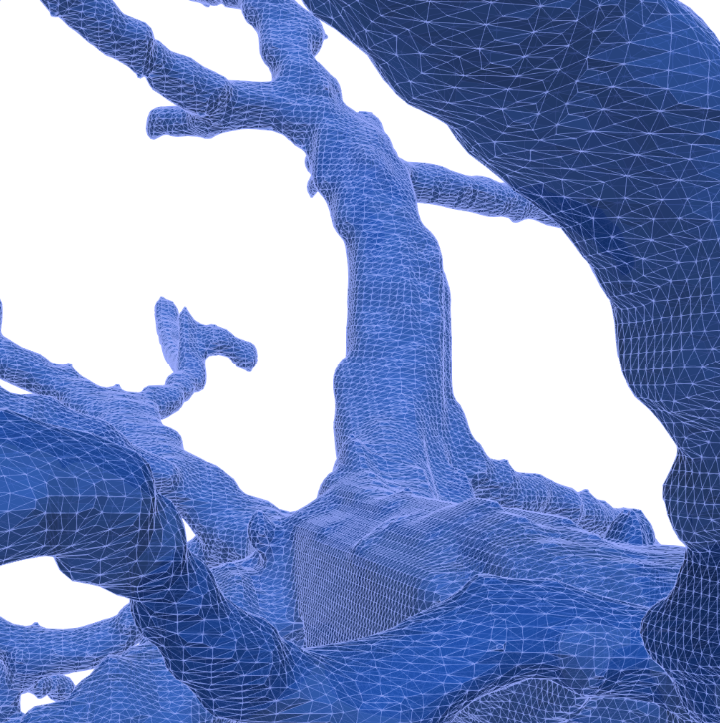
\includegraphics[height=0.3\textwidth,width=0.33\textwidth]{figs/image-1.png}%
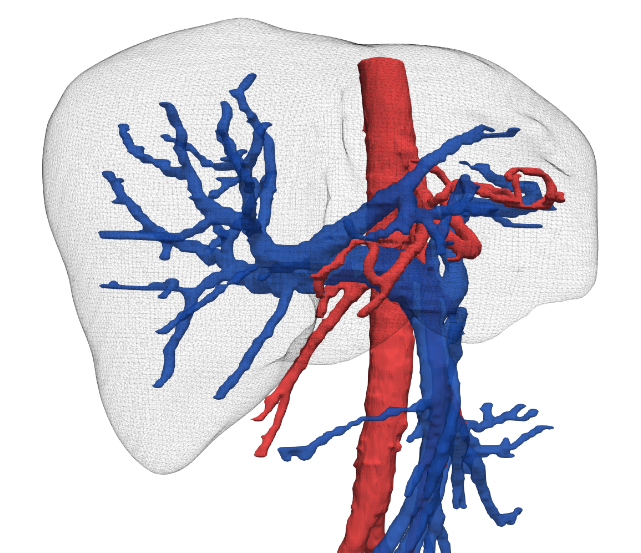
\includegraphics[height=0.3\textwidth,width=0.33\textwidth]{figs/image-2.png}%
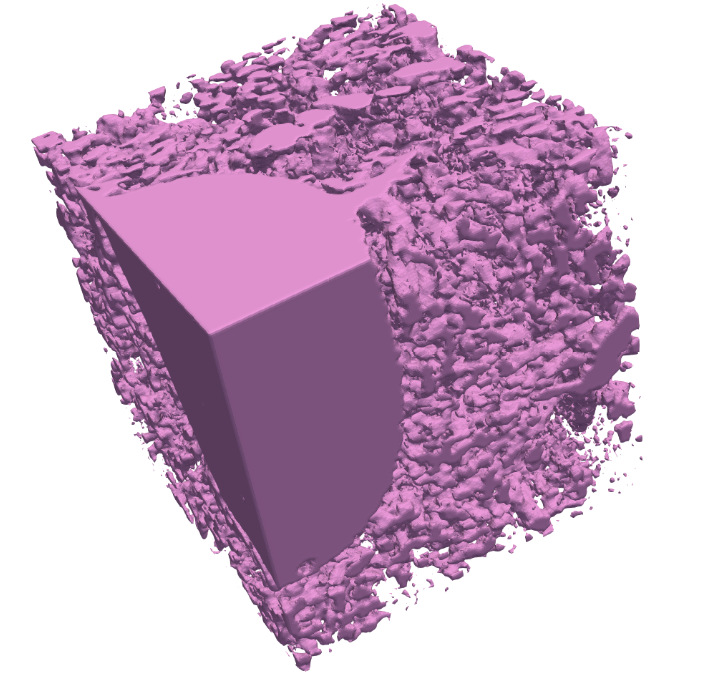
\includegraphics[height=0.3\textwidth,width=0.33\textwidth]{figs/image-3.png}%
\caption{Images of human liver: (a) portal vein (PV); (b) frontal view, showing also the part of PV connected to the colon and stomach; (c) interlobular veins. Note that brick boundaries look flat.}
\label{fig:schema}
\end{figure}


\newpage

\vspace{10pt}
\noindent\underline{
Conclusion:
}\vspace{0.2em}\newline 
We introduced a Julia implementation of an algebraic filter to extract from 3D medical images the
boundary surface of some specific image segment, described as a 3-chain of voxels. Translations from
Cartesian indices of cells to linearized indices, the computation of the sparse boundary matrices, and the
sparse matrix-vector multiplication are the main computational kernels of this approach. 

% NEW next two sentences are new
We may show a good speed-up over marching-cubes algorithms. 
The existing implementation employs Julia's channels
for multiprocessing. 
Parallelization makes a large portion of spared computational cost. 
%
Moreover, we expect additional improvement in the future because our approach is appropriate  for SIMD (Single Instruction, Multiple Data) hybrid architectures of CPUs and GPUs, since only the initial block setup of boundary matrix and image slices, as well the final collection of computed surface portions, require inter-process communication. 

\sloppy{
Currently, the computational pipeline is being strongly improved to gain a greater
speed-up using native Julia implementation \texttt{CUDA.jl} of Nvidia programming platform 
% TODO cite Besard2017 [7]
% \cite{Besard:2017}
\cite{Besard2019}
, and Julia's
\texttt{SuiteSparseGraphBLAS.jl} framework 
\cite{Buluc2017}
% TODO cite BULUK 2017 [8] 
for graph algorithms with the language of linear algebra. In
particular, we are extending its use pattern in order to work with general cellular complexes.
}


%%%%%%%%%%%%%%%


% \section{Neni moje}


% In engineering workflows it is common practice to maintain master CAD geometries, which then serve as a foundation for further design and development. Preserving CAD parametrisations during aerodynamic shape optimisation becomes challenging since existing CAD tools do not provide derivatives necessary for gradient-based design methods. Hence, gradients are obtained by approximations or with simplifications, precluding full CAD integration into the design optimisation loop.

 
% In the present work, we obtain exact CAD sensitivities (derivatives) with respect to CAD design parametrisation using our algorithmically differentiated Open Cascade Technology (OCCT) CAD-kernel software.  The extension of this software for optimisation of parametric models and BRep (NURBS) compose the tool for explorations of the optimal shape in different by size and nature design spaces. In addition, we demonstrate the imposition of geometric constraints for both approaches, a salient part of industrial design, and an intuitive method of storing them in standard CAD format.\newline


% \textbf{This template file is courtesy of Orest Mykhaskiv, Jens-Dominik M\"uller, Pavanakumar Mohanamuraly, Mladen Banovic, Andrea Walther, Salvatore Auriemma and Herve Legrand.}


% \vspace{10pt}
% \noindent\underline{CAD-based Shape Optimisation:}\vspace{0.2em}\newline
% To assess the aerodynamic performance of a given CAD geometry with design parameters $\alpha$, one usually computes a scalar cost function $J$ (drag, lift, total pressure loss, etc.) on the corresponding computational mesh.  In order to obtain a shape with improved characteristics we consider an optimisation problem \cite{jameson88aerodynamic}:       
% \begin{equation}
% \label{eq:cost-func}
% \underset{\alpha}{min} \hspace{0.5em} J(U(X(\alpha)), X(\alpha), \alpha)
% \end{equation}
% \begin{equation}
% \label{eq:NS}
% R(U(X(\alpha)), X(\alpha)) = 0\:. 
% \end{equation}
% Equation \eqref{eq:NS} describes the flow field within the domain of interest by system of Reynolds-Averaged Navier-Stokes equations, with the state variable $U$ and computational mesh coordinates $X$, which depend on design parameters $\alpha$. In case of large amount of design parameters (usually the case in industrial applications) the adjoint method proves to be computationally efficient and could be derived by application of a chain rule to the system \eqref{eq:cost-func}-\eqref{eq:NS} yielding:
% \begin{equation}
% \label{eq:sens}
% \dfrac{dJ}{d\alpha}=\Big[ \frac{dJ}{dX} +\nu^Tf \Big]\frac{\partial X}{\partial \alpha}\:,
% \end{equation}
% where 
% \begin{equation}
% f = -\frac{\partial R}{\partial X}\:.
% \end{equation}
% Here $\nu$ represents the solution of adjoint equations:
% \begin{equation}
% \label{eq:adjoint}
% \Big ( \frac{\partial R}{\partial U}\Big)^T\nu=\frac{\partial J}{\partial U}\:.
% \end{equation}
% After computing the solution of primal and adjoint equations \eqref{eq:NS},\eqref{eq:adjoint}, one can rewrite cost function gradient in terms of surface grid points derivatives:
% \begin{equation}
% \label{eq:surfSens}
% \frac{dJ}{d\alpha}=\frac{dJ}{dX_S}\frac{dX_S}{d\alpha}\:.
% \end{equation}
% Here, the relation (spring analogy, inverse distance weighting) between volume and surface grid points displacement is used $X = X(X_S)$. 
% The first term in \eqref{eq:surfSens}, usually called \textit{CFD sensitivity}, corresponds to the flow sensitivity in the surface grid points $X_S$. These derivatives could be calculated by several available CFD solvers that have implemented the adjoint method. In this work we use our in-house discrete adjoint solver STAMPS (previously \textit{mgopt}) \cite{xu2015thesis}. 

% The second term (\textit{CAD sensitivity}) represents the derivative of the surface grid points $X_S$ with respect to the CAD model design parameters. This part is calculated in the automatically differentiated version of OCCT \cite{auriemma2016optimisation}. Although the process of differentiation of the complete CAD system was time-consuming and involved comprehensive code modifications (due to the size and complexity of the software), the final result is extremely beneficial for the CAD-based optimisation. The differentiated OCCT provides the derivatives for almost every possible CAD parametrisation and geometrical manipulation. 

% Equipped with these derivatives, we compose them in the total gradient, which is then used in iterative gradient-based optimisation loop:
% \begin{equation}
% \alpha^{(n+1)} =  A\big(\alpha^{(n)}, \frac{dJ}{d\alpha}(\alpha^{(n)})\big) \:,\end{equation}
% with $A$ as an optimisation algorithm. 
% Next sections describe two cases of the above mentioned method, depending on the nature of CAD design parameter $\alpha$: as design variable in parametric CAD model or BRep/NURBS parametrisation.



% \vspace{10pt}
% \noindent\underline{Parametric CAD-model Optimisation:}\vspace{0.2em}\newline
% Parametric models are extremely popular in industry since they allow designers and engineers to map their intuition and experience on a set of familiar and conventional variables: e.g. blade thickness, fillet radius, wing span, etc. The OCCT kernel proposes large amount of methods for typical parametric model construction: starting from sketches with pre-defined sizes, construction of 2D curves to further 3D shapes manipulations, boolean operations, etc. The software architecture of the differentiated OCCT allows to build parametric models with no difference to the original version, but additionally is capable of providing the derivatives with respect to the used design parameters. 

% Existence of a parametric CAD model creates a natural way to incorporate various geometrical constraints, since most of design variables are explicitly controlled by user-defined parametrisation. In the final paper, an example of parametric CAD model in differentiated OCCT will be presented (TU Berlin Stator testcase, see description below), as well as the results of aerodynamic shape optimisation subject to several geometrical constraints. 


% \vspace{10pt}
% \noindent\underline{BRep (NURBS-based) Optimisation and Constraints:}\vspace{0.2em}\newline
% Alternatively to the previous section, instead of changing the parameters of the model's construction algorithm, one can directly modify the geometry of the resulting shape, so-called BRep (Boundary Representation). Changes to this BRep data (control points positions and weights of corresponding NURBS) eliminate the initial parametrisation, but propose richer design spaces compared to sometimes limited parametric models. Hence, this method serves better the ultimate goal of optimisation, potentially exploring non-conventional designs. The method is CAD-vendor independent, and requires only a generic CAD-file (STEP, IGES, etc.), eluding problems with parametrisation tree and making the optimisation more automatic. With method implementation in OCCT, one can easily and intuitively refine design space by adding extra control points. 
% \begin{figure}[t!]
% \label{fig:constraint}
% \begin{center}
% \includegraphics[width = 0.3\textwidth]{images/NewCylindersC1.pdf}
% ~~

% \includegraphics[width = 0.6\textwidth]{images/const3.pdf}
% \caption{Left: Constraint visualisation from the STEP file; Right: Constraints computation on the testpoints}
% \end{center}
% \end{figure}

% CAD models are usually constructed from multiple adjacent patches. Therefore, modifications of control points individually on patches can violate (i) patch-continuity (holes between the CAD faces, non-smooth shapes) or (ii) other geometrical constraints. We alleviate this problem by filtering out the shape modes with undesired constraints violations using discrete spaces constructed using test-points (NSPCC approach) \cite{xu13:cad-based},\cite{xu15cad-based}. Conceptually, the approach requires that the constraints are satisfied on the particular set of points defined on the surface (test-points). 

% In this work, we propose further development of NSPCC for user-friendly constraints definition. Several methods were devised to accelerate and automate the process of test-point distribution and visualise them.  In Fig. 1. the constraints are deployed in pairs and stored in a coloured STEP format. On each coloured pair, a number of test-points are distributed by means of OCCT, and then composed in the constraint matrix as in \cite{xu15cad-based}. Making use of the OCCT functionality and its differentiated version, the following types of constraints are implemented and also presented in Fig.1.:
% \begin{itemize}
% \item Cross-patch continuity ($C_{d1}$)
% \item Distance $(C_{d2}, C_{d3})$
% \item Distance in X, Y, or Z direction
% \item Radius of curvature in some point ($C_{r1}, C_{r2}$)
% \end{itemize}
% In the next section, the results of NURBS-based optimisation with above-mentioned constraints are shown.


% \vspace{10pt}
% \noindent\underline{Results for the TU Berlin Stator Testcase:}\vspace{0.2em}\newline
% The complete description of TU Berlin Stator testcase could be found via \url{http://aboutflow.sems.qmul.ac.uk/events/munich2016/benchmark/testcase3/}. This case represents a typical turbomachinery optimisation problem, subject to a number of geometrical constraints. The corresponding constraint file is shown in Fig. 1. and includes minimal thickness constraint in the middle of the blade, spaces for four bolts (two at the hub and two at the shroud sides), axial chord constraint (Distance in X) and minimal radius for the trailing and the leading edge (Radius of curvature constraint).

% \begin{figure}[t!]
%   \centering
%     \includegraphics[width=0.5\textwidth, height=200px]{images/blades}
%     ~~~
%     \includegraphics[width=0.45\textwidth, height = 180px]{images/costFunction}
% 	\caption{Left: Original and Optimised TUB stator blade with NURBS Control Point Net; Right: 20 iterations of Optimisation loop}
%     \label{fullmodel}
% \end{figure}



% With all constraints set, the optimisation is conducted with NSPCC approach to minimise the total pressure loss in the stator at the operating point with 42 degrees of swirl. The results are provided in Fig. 2. and were obtained on the coarse mesh with the STAMPS solver and differentiated OCCT. The changes of NURBS control point net resulted in partial shrinking of the blade, while NSPCC methodology prevented an infraction of the constraints, in general providing 18\% improvement to the cost function.   


% \vspace{1em}
% \noindent\underline{Conclusions:}\vspace{0.2em}\newline
% The use of differentiated CAD-kernel OCCT in combination with adjoint CFD method is showcased for the aerodynamic shape optimisation. The developed CAD tool allows to find optimised designs  and impose geometrical constraints for both parametric models and generally richer NURBS parametrisation spaces with result directly in the CAD format. In the final paper NURBS-based optimisation will be enhanced by automatic design space refinement and it will be compared to a parametric optimisation where the design space consists of conventional turbomachinery parameters.

\vspace{1em}
\noindent\underline{Acknowledgement:}\vspace{0.2em}\newline
\sloppy{
This work was supported by Charles University Research Centre program UNCE/MED/006 ``University Center of Clinical and Experimental Liver Surgery'' and Ministry of Education project ITI CZ.02.1.01/0.0/0.0/17\_048/0007280: Application of modern technologies in medicine and industry.
} 
% The research was also supported by the project LO 1506 of the Czech Ministry of Education, Youth and Sports.

% \vspace{1em}
% \noindent\underline{IMPORTANT NOTES:}\vspace{0.2em}\newline
% WE ARE REQUIRED BY CROSSREF TO INCLUDE HYPERLINK INTO EVERY REFERENCE THAT HAS DOI LINKING. PLEASE GO TO: \ULurl{http://www.crossref.org/SimpleTextQuery/}, REGISTER YOUR E-MAIL, CUT AND PASTE THE LIST OF REFERENCES INTO THE BOX, GET THE DOI LINKS AND PASTE THEM INTO YOUR PAPER! THE LINKS SHOULD LOOK LIKE THIS, I.E. USE HTTPS AND DROP THE DX: \ULurl{https://doi.org/10.1080/16864360.2014.881190}


\vspace{1em}
\noindent\underline{References:}\vspace{-1.9em}\newline
\renewcommand{\section}[2]{}

% \bibliographystyle{alpha}
\bibliographystyle{cadp2020}
\bibliography{TSAS-2019,references}
\small

% \begin{thebibliography}{9}
% \bibitem{auriemma2016optimisation}Auriemma, S.; Banovic, M.; Mykhaskiv, O.; Legrand, H.; M\"uller, J.-D.; Walther, A.: Optimisation of a U-bend using CAD-based adjoint method with differentiated CAD kernel, ECCOMAS Congress, 2016.

% \bibitem{jameson88aerodynamic} Jameson, A.: Aerodynamic Design via Control Theory, Journal of Scientific Computing, 3, 1988,  233--260. \ULurl{https://doi.org/10.1007/BF01061285}

% \bibitem{xu2015thesis} Xu, S.: CAD-based CFD shape optimisation using discrete adjoint solvers, Ph.D. Thesis, Queen Mary University of London, 2015.

% \bibitem{xu15cad-based} Xu, S.; Radford, D.; M\"uller, J.-D.: CAD-based adjoint shape optimisation of a one-stage turbine with geometric constraints, ASME Turbo Expo, 2015.

% \bibitem{xu13:cad-based} Xu, S.; Wolfram, J.; M\"uller J.-D.: CAD-based shape optimisation with CFD using a discrete adjoint, International Journal for Numerical Methods in Fluids, 74(3), 2013, 153-168. \ULurl{https://doi.org/10.1002/fld.3844}
% \end{thebibliography}



\end{document}
